\documentclass{intech}
 
%\usepackage{your_package}	%if you need custom package
%\usepackage[notquote]{hanging}
 

% * CHAPTER NUMBER * BOOK NAME * AUTHOR(S) NAME *****************************
\setcounter{chapter}{0} % It will be set by technical editor.

\booktitle{Wireless Energy Transfer  based on Electromagnetic Resonance: Principles and Engineering Explorations}%

\chaptertitle{The Phenomenon of Wireless Energy Transfer: Experiments and Philosophy} % You know your chapter title?

\authors{H. V\'azquez-Leal, A. Gallardo-Del-Angel, R. Casta\~neda-Sheissa and F. J. Gonz\'alez-Mart{\'i}nez}
\affiliation{Universidad Veracruzana \\ Facultad de Instrumentaci\'on Electr\'onica}
\country{M\'exico}

% uncomment the next three or six lines, when authors are from diferent university, company or country

%\secondauthors{Author(s) with another affiliation}
%\secondaffiliation{Name of the 2nd University (Company)}
%\secondcountry{2nd country}

%\thirdauthors{}
%\thirdaffiliation{}
%\thirdcountry{}

% END * CHAPTER NUMBER * BOOK NAME * AUTHOR(S) NAME *************************


\begin{document}

\maketitle

\section{Introducci\'on}


En la termodin\'amica existe una ley b\'asica; la ley de la conservaci\'on de la energ{\'i}a, la cual dice escencialmente que: {\it La energ{\'i}a no se crea ni se destruye s\'olo se transforma}. La naturaleza es experta en usar esta ley fundamental de la f{\'i}sica a favor
de la vida y la evoluci\'on de las especies en nuestro planeta, se puede decir que estamos tan acostumbrados a 
vivir regidos por esta ley, que no nos percatamos de su existencia e influencia en nuestras vidas. 

Desde el origen de la humanidad el hombre ha usado la energia de la naturaleza a su favor. Cuando
descubrio el fuego lo primero que intento hacer es trasladarlo desde lo encontraba hasta sus refugios.
Mas tarde, el hombre aprendio a recolectar y transportar combustibles  como el carbon mineral, carbon vegetal, entre otros, mismos que transformaba en calor y/o luz. De hecho el transporte de la energia se hizo tan
importante para la construccion de sociedades que cuando la energia electrica fue inventada, rapidamente
se construyo la red de transporte de energia mas grande y sofisticada que aun conoce la humanidad actual, las redes de distribucion de energia electrica. Dichas redes de distribucion impulsaron grandes avances en la ciencia orientados
a optimizar la efiencia en el transporte de dicha energia. Sin embargo, es comun que se pierda el 30\%
de la energia por diversas razones. Actualmente, existen aplicaciones de uso practico en las que una forma de transporte de energia sin cables es mas conveniente entre las que se pueden mencionar:

\begin{itemize}
\item Implantes biomedicos. El avance en la ciencia de la bioelectronica a permitido
crear implantes biomedicos como: marcapasos, implante coclear, suministradores subcutaneos de medicamento, entre otros.
\item Carga de dispositivos mobiles, autos electricos, aviones no tripulados, entre otros.
\item Electrodomesticos como planchas, aspiradoras, televisores, entre otros.
\end{itemize}

Dichas aplicaciones potenciales han impulsado el interes por
la transferencia inal\'ambrica de energ{\'i}a. Sin embargo, la naturaleza siempre un paso adelante de nosotros, ya tiene {\it tiempo} transfiriendo y transformado la energ{\'i}a sin utilizar un s\'olo cable de cobre. La fuente de energ\'{i}a inal\'ambrica
m\'as grande existente en nuestro planeta es la solar; la naturaleza aprovecha la luz del sol mediante el proceso de la fotosintesis,
generando asi los nutrientes que m\'as tarde se convierten en motor de la cadena alimenticia y de la vida.  
Actualmente, se han inventado diversas formas de convertir la luz del sol en energ{\'i}a el\'ectrica, entre ellas, la m\'as famosa es la de las celdas fotovoltaicas. Sin embargo, la recoleccion de la energia solar
es solo el primer paso, luego el distribuir la energia en las zonas donde se usara la otra parte
del problema, es decir,  el nuevo objetivo es transferir inalambricamente punto a punto la energia.


Esta nueva tendencia tecnol\'ogica hacia la energ{\'i}a inal\'ambrica, no es tan nueva
como se podr{\'i}a pensar. Ya se sabe que el verdadero inventor de la radio fue Nikola Tesla, por lo tanto, resulta logico
pensar que ese mismo cientifico infiriera, que si era posible  transferir informacion por campo electromagnetico, tambien
deberia ser posible transferir potencia por el mismo medio.  Por lo tanto, a principios del siglo 19 el destacado cient{\'i}fico e inventor realiz\'o experimentos (\cite{RES20}) sobre transferencia inal\'ambrica de energ{\'i}a logrando resultados asombrosos para su \'epoca.
Se dice que con los experimentos de tesla se alcanzo a  iluminar lamparas a 40kms de distancia.
Sin embargo, por lo peligroso de los experimentos, la baja eficiencia en la transferencia de potencia, y principalmente por el agotamiento de sus recursos financieros, Tesla abandon\'o los experimentos, quedando su legado en forma de una patente que nunca explot\'o comercialmente. 


La radiaci\'on electromagn\'etica  se ha utilizado t{\'i}picamente para la transmisi\'on inal\'ambrica de informaci\'on.
 Sin embargo, la informaci\'on viaja en ondas electromagn\'eticas las cuales son finalmente una forma de energ{\'i}a. Por lo tanto,
 en teor{\'i}a es posible la transmisi\'on de energ{\'i}a de una manera similar
 a la utilizada para transferir informaci\'on (voz y datos). En particular, se puede alcanzar a transferir de manera direccional grandes potencias con el uso de las microondas (\cite{RES22}). Aunque el m\'etodo es eficiente, tiene dos desventajas: requiere de l{\'i}nea de vista y es un mecanismo peligroso para los s\'eres vivos. Por lo tanto, la  transferencia inal\'ambrica de energ{\'i}a  por medio del fen\'omeno de resonancia electromagn\'etica
se ha convertido en una opci\'on viable, almenos para distancias cortas, ya que tiene una alta eficiencia
en la trasnferencia de potencia.

Actualmente se ha transferido energ{\'i}a de forma inal\'ambrica usando diversos mecanismos f{\'i}sicos como lo son: 

\begin{itemize}
\item Laser. El rayo laser es un haz coherente de luz capaz de transportar muy altas energ{\'i}as, lo que lo convierte en un mecanismo eficiente para mandar energ{\'i}a de punto a punto en l{\'i}nea de vista. La NASA (\cite{RES21}) present\'o en 2003 un avi\'on teledirigido energizado de manera inal\'ambrica con un rayo laser y una celda fotovoltaica sensible al infrarrojo funcionando como recolector de energ{\'i}a. De hecho la NASA est\'a proponiendo dicho esquema para energizar sat\'elites y transmisi\'on inal\'ambrica de energ{\'i}a donde ning\'un otro mecanismo sea viable (\cite{RES21}).
\item Principio piezoel\'ectrico (\cite{RES8}). Se ha demostrado que es posible transferir energ{\'i}a de manera inal\'ambrica mediante el uso de transductores piezoel\'ectricos capaces de emitir y recolectar ondas vibratorias.
\item Ondas de Radio y Microondas. En \cite{RES22} se muestra como transmitir energ{\'i}a de alta potencia a grandes distancias usando Microondas . Adem\'as, existe todo un campo de investigaci\'on en el \'area de rectenas \cite{RES4,RES9,RES10,RES12} las cuales son antenas capaces de recolectar energ{\'i}a de las ondas de radio.
\item Acoplamiento inductivo (\cite{RES3,RES5,RES6,RES7}). El acoplamiento inductivo funciona bajo el efecto de acoplamiento resonante entre las bobinas de dos circuitos LC. La eficiencia m\'axima eficiencia s\'olo se alcanza cuando el transmisor y el receptor se encuentran a muy corta distancia.
\item Resonancia electromagn\'etica "fuerte". En (\cite{RES1,RES2}) se present\'o m\'etodo de transferencia inal\'ambrica de energ{\'i}a, el cual usa el fen\'omeno de resonancia electromagn\'etica "fuerte", logrando transferir energ{\'i}a de manera eficientemente a varias decenas de cent{\'i}metros.
\end{itemize}

Transferir grandes cantidades de potencia por medio de campo electromagnetico, crea inevitablemente la inquietud
sobre los efectos nocivos que esto pueda traer a la salud. Por lo tanto, en la siguiente seccion se abordara
un brevemente sobre la literatura cientifica al respecto.


\section{Ondas electromagn\'eticas y la salud}

Desde el descubrimiento de las ondas electromagneticas se inicio una carrera tecnologica para aprovechar las ventajas de transferir informacion de manera inalambrica. La carrera tecnologica se inicio con la transmision de  codigos Morse, pero rapidamente llego la radio, television, los celulares y las versiones digitales de todos los antes mencionados; A lo dicho anteriormente se sumaron en la ultima decada
un sinfin de dispositivos moviles con capacidades comunicacion inalambrica, mismos que se usan de manera masiva por la población. Como resultado de lo anterior, es comun que
una persona promedio se vea sometida constantemente a los campos electromagneticos en frecuencias que abarcan desde los MHz hasta los GHz. Por lo tanto, la poblaci\'on se encuentra cada d{\'i}a m\'as preocupada por los efectos en la salud debido a la exposici\'on a toda la radiaci\'on electromagn\'etica que hoy d{\'i}a produce nuestra sociedad. Ademas, ahora se suma al debate la preocupacion
por los mecanismos de transferencia inal\'ambrica de energ{\'i}a que trabajan con se\~nales electromagn\'eticas.

Se han realizado diversos estudios (\cite{RES15,RES16})  sobre los efectos de las ondas electromagn\'eticas, en particular las de los celulares, comprob\'andose que justo en los l{\'i}mites de seguridad internacionales existen ciertos efectos en los genes. En (\cite{RES13}) se asegura que no es posible aun, determinar que existan efectos en la salud a corto o largo plazo  debido a exposici\'on a ondas electromagn\'eticas c\'omo las emitidas por estaciones de transmisi\'on y telefon{\'i}a Celular. Sin embargo, en (\cite{RES14}) se realiz\'o un estudio con 10,497 marines de la Royal Norwegian Navy; El resultado para quienes trabajaron en la cercan{\'i}a de 10m de estaciones transmisoras o radares, fue un incremento en la infertilidad, y una mayor tasa de nacimientos mujeres que de hombres.
El incremento de infertilidad concuerda con otro estudio (\cite{RES14x}) que determino que la calidad del semen disminuye en los hombres que por razones laborales (electricistas, t\'ecnicos, soldadores, etc) son expuestos a la radiaci\'on electromagn\'etica constante incluyendo las microondas.  Los estudios realizados demuestran que si existen algunos efectos  en los seres humanos.

\section{Resonancia Ac\'ustica y El\'ectrica}

La resonancia mec\'anica o ac\'ustica es bien conocida en la f{\'i}sica y consiste en aplicar a un objeto una acci\'on vibratoria peri\'odica cuyo periodo de vibraci\'on coincide con la frecuencia en la que el objeto tiene la mayor tasa de absorci\'on de energ{\'i}a. A dicha frecuencia se le conoce como frecuencia de resonancia. 
Este efecto puede ser destructivo en algunos materiales rigidos como el vaso que se rompe cuando un tenor canta,
o en caso mas extremos hasta un puente o un edificio pueden derribarse por la resonancia, sea esta provocada por el viento
o por temblores.

La resonancia es bien conocido en la mec\'anica, pero tambien existe en la electricidad y se conoce como resonancia el\'ectrica o inductiva. Dicho fen\'omeno se puede utilizar para transferir energ{\'i}a de manera inal\'ambrica con dos ventajas principales: se garantiza m\'axima  tasa de absorci\'on de energ{\'i}a  y se puede trabajar a frecuencias bajas (menos peligrosas para el ser humano). Cuando dos objetos tienen la misma frecuencia de resonancia estos se pueden acoplar de manera resonante de tal modo que un objeto le puede transferir energ{\'i}a (de manera eficiente) al otro. Este principio se puede aprovechar para transmitir energia 
de un punto a otro, por
medio de campo electromagnetico. A continuaci\'on se describen tres mecanismo de transferencia inal\'ambrica de energ{\'i}a:

\begin{enumerate}
\item {\bf El acoplamiento inductivo (\cite{RES3})}  es el acoplamiento resonante que existe entre las bobinas de 2 circuitos $LC$ con la misma frecuencia de resonancia, transfiri\'endose energ{\'i}a de una bobina a la otra como se ve en la figura \ref{fuerte}. La desventaja de esta t\'ecnica es que la eficiencia se pierde r\'apidamente con la separaci\'on entre las bobinas. 
\item {\bf El acoplamiento auto-resonante fuerte (\cite{RES1})}. La auto-resonancia existe de manera natural en todas
las bobinas ($L$), aunque, esta frecuencia ($f_r=1/(2\pi \sqrt{L C_p})$) es normalmente demasiada alta debido a que la capacitancia parasita ($C_p$) es muy baja. Sin embargo en  (\cite{RES1})
se demostr\'o que es posible lograr una buena eficiencia con un esquema como el mostrado en la figura \ref{fuerte}(b). 
Para que el acoplamiento supere el 40\% reportado en \cite{RES1} el radio  ($r$) de la bobina debe ser mucho menor que la longitud de onda ($\lambda$) de la frecuencia de resonancia y la separacion ($d$) optima para un buen acoplamiento se tal que $r\ll d\ll \lambda$, de tal modo que el acoplamiento es proporcional a $(\frac{r}{\lambda}\frac{r^3}{d^3})$
(\cite{meta}).
Existen 2 diferencias fundamentales con el acoplamiento inductivo simple de la figura \ref{fuerte}(a) es: 
la capacitancia del circuito LC es par\'asita y no discreta, y ahora las bobinas ($T$ y $R$) estan acopladas a otro par de bobinas $L_S$ y $L_L$ de una s\'ola espira, las cuales actuan fuente emisora de la energ{\'ia} y bobina receptora de la energ{\'i}a respectivamente. La frecuencia de auto-resonancia en una bobina depende de su capacitancia par\'asita, por lo que normalmente dicha frecuencia es muy alta (orden de Ghz). Por lo tanto, para alcanzar una frecuencia de auto-resonancia baja ($<10$Mhz) es necesario usar alambre de cobre grueso y espaciado con la finalidad de lograr una capacitancia parasita grande y as{\'i} reducir la frecuencia de auto-resonancia al orden de los megahertz. De hecho, en \cite{RES1,RES2} se reporta un experimento con cable de radio de 3cm.
La eficiencia en la transferencia de potencia en funci\'on de la distancia tiene una relaci\'on inversamente
proporcional al radio de la bobina, y es por esta raz\'on, que en los experimentos reportados en \cite{RES1}\cite{RES2} las bobinas tienen radios de 30cm.
\item En la figura \ref{fuerte}(c) se muestra un esquema de acoplamiento que podriamos denominar {\bf "acoplamiento resonante inductivo fuerte"}, el cual es una modificaci\'on del acoplamiento resonante fuerte (Ver figura \ref{fuerte}(b)). La modificaci\'on
consiste en cambiar la capacitancia par\'asita $C_p$ por una capacitancia discreta $C$. De esta manera, se elima la necesidad
de usar cable de grueso calibre y grandes dimensiones.
\end{enumerate}
\begin{figure}[htbp]	% H-must be here or [htb]
\centering
\subfigure[Inductive resonant coupling]{\includegraphics[width=7.3cm]{./img/acoplamientos-1.eps}} %	** if .eps don't need extension
\hspace{0.5cm}
\subfigure[Strong self-resonant coupling]{\includegraphics[width=7.7cm]{./img/acoplamientos-2.eps}}
\hspace{0.5cm}
\subfigure[Modified inductive resonant coupling]{\includegraphics[width=8cm]{./img/acoplamientos-3.eps}} %	** if .eps don't need extension
\vspace{-0.5cm}
\caption{Coupling schemes}
\label{fuerte}
\end{figure}


\section{Experimentaci\'on}

Se utilizaran bobinas triangulares y circulares para establecer un acomplamento resonante inductivo tal y como se  muestra en la figura \ref{circutriangular}.

\begin{enumerate}
\item {\bf Acoplamiento resonante inductivo}. Este experimento fue dise\~nado (\cite{SOMI}) con la finalidad de visualizar el patr\'on de radiaci\'on y eficiencia
de un acoplamiento resonante inductivo. Primero se mantuvo la bobina generadora en una posici\'on fija mientras
que la bobina receptora ($R$) gira alrededor de la bobina generadora ($T$), a una distancia fija y con desplazamiento angular constante completando 360 grados (Ver Figura \ref{datos1}). De este experimento se observa que la energ{\'i}a producida por la bobina transmisora $T$ se propaga a 90$^\circ$ frente a la bobina generadora y a 90$^\circ$ atr\'as de la misma. En otra etapa del experimento se colocaron las dos bobinas de manera paralela y conc\'entrica a una distancia de cero cent{\'i}metros y se procedio a alejarlas. Los
resultados se muestran en la figura \ref{datos1}(c). Se puede observar claramente que la eficiencia m\'axima en ganancia de voltaje es del  50\% (a cero centimetros). Lo cual es l\'ogico
al observar el patr\'on de radiaci\'on  en la figura \ref{datos1}(b), ya que ex{\'i}ste un lobulo trasero de radiaci\'on desperdiciado. En la figura \ref{datos1}(c) se muestra como, m\'as all\'a de una distancia de 8 cm, la ganancia en voltaje del sistema cae por debajo del 5\%. El l\'obulo trasero puede ser reaprovechado utilizando una superficie reflectora del campo electromagn\'etico.
\begin{figure}[htbp]	% H-must be here or [htb]
\centering
\subfigure[Proceso del experimento de rotaci\'on de bobina receptora]{\includegraphics[width=7cm]{./img/coil3d.eps}} %	** if .eps don't need extension
\subfigure[Patron de radiaci\'on]{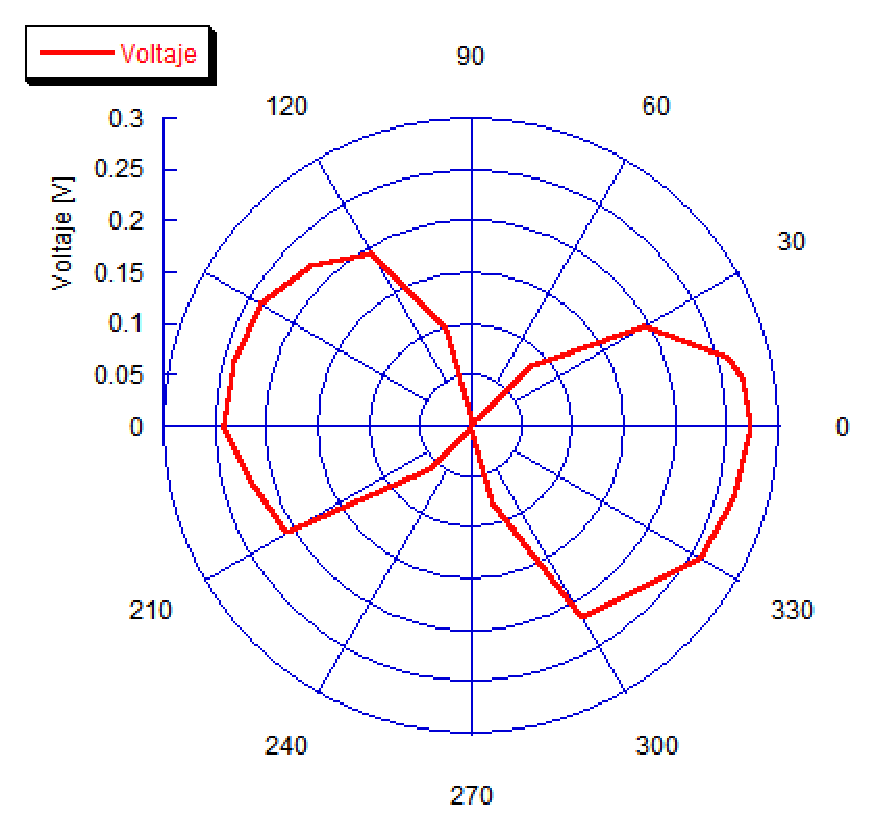
\includegraphics[width=7cm]{./img/image1a.eps}}
\subfigure[Ganancia en voltaje del sistema con relaci\'on de voltajes]{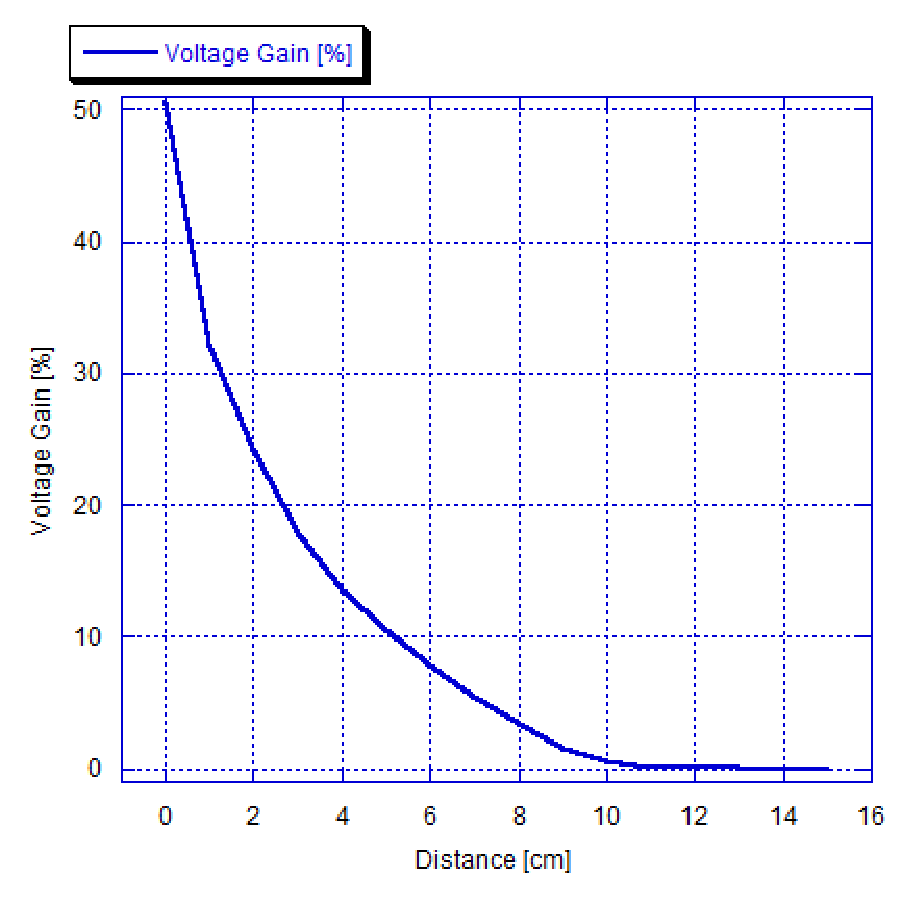
\includegraphics[width=6cm]{./img/image2.eps}} %	** if .eps don't need extension
\caption{Patr\'on de radiaci\'on de la bobina generadora a  1.4MHz}
\label{datos1}
\end{figure}
\item  {\bf Bobina triangular}. En la versi\'on extensa de este trabajo se presentar\'a los dos experimentos anteriores realizados con bobinas triangulares. Adem\'as,
se realizar\'a una comparaci\'on con los resultados de los experimentos 1  y 2.
\end{enumerate}
\section{Filosof{\'i}a}
La energ{\'i}a inal\'ambrica de: alta potencia (>100W), a distancias moderadas (>10M), de buena eficiencia (>70\%), sin riesgos de salud y de bajo costo; Es un sue\~no que hoy d{\'i}a sostiene la atenci\'on de investigadores al rededor del planeta. 
Sin embargo, para que todo sue\~no se materialize se requiere de ideas innovadoras o inclusive totalmente radicales, que den respuesta  a las grandes interrogantes que se oponen a la meta. Por lo tanto, se requiere de innovaciones en las siguientes direcciones:
\begin{itemize}
\item Bobinas de geometr{\'i}as diferentes. Las bobinas utilizadas para los experimentos reportados en casi toda la literatura son una simple espiral.  Sin embargo, se pueden usar nuevas geometr{\'i}as que cambien el patron de radiaci\'on
del campo electromagn\'etico, en la busqueda de aumentar: direccionalidad, distancia y/o eficiencia.
Con bobinas totalmente diferentes, como las triangulares, exagonales, multiformes, se podria generar patrones de radiaci\'on altamente no lineales como los mostrados en la figura  \ref{patronloco}.
\begin{figure}[hbtp]
\centering
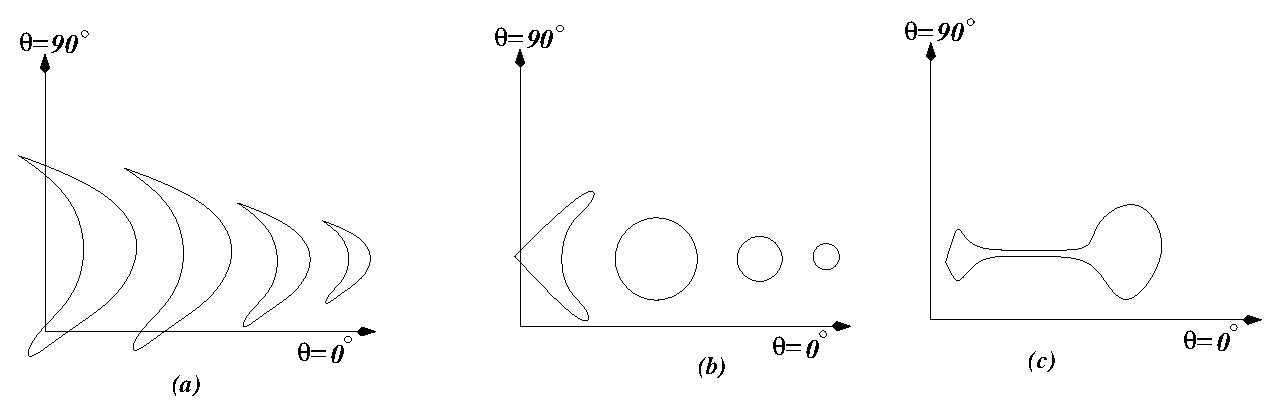
\includegraphics[width=12cm]{img/patrones.eps}
\caption{Nuevos patr\'ones de radiaci\'on}
\label{patronloco}
\end{figure}
\item El uso de nuevos materiales para mejorar la eficiencia. Por ejemplo, se podria emular la autoresonancia de las bobinas
del experimento 2, mediante una bobina-capacitor. Esta bobina estar{\'i}a dise\~nada de tal forma que entre cada espiria quedar{\'ia} un material diel\'ectrico, de tal manera que se crear{\'i}a un capacitor parasito a lo largo de todas las espiras de la bobina. Por lo tanto, se generar{\'i}a una capacitancia parasita lo suficientemente grande como para lograr una autoresonancia en el orden de los MHz.
La ventaja de esta bobina-capacitor es que no se requerir{\'i}a bobinas con cable de gran grosor y espaciado entre las espiras.
\item En (\cite{meta}) se demosotro que el uso de metamateriales puede mejorar el desempeño de sistemas acoplados resonantemente en campo cercano. They proposed a power relay system based on a near-field metamaterial superlens.
Este es un primer paso rumbo a la optimizacion del fenomeno de acoplamiento resonante en campo cercano,
el siguiente sera el diseño de bobinas implementadas con metamateriales en la busqueda de afectar direccionalidad
o eficiencia.
\item Sistemas multiresonantes acoplados inductivamente. El uso de bobinas amorfas o multiformes podr{\'i}a generar m\'ultiples frecuencias de resonancia
que dependiendo de su distribuci\'on y grado de eficiencia, se utilizar{\'i}an para transferir energ{\'i}a de manera simultanea por m\'as de una frecuencia de resonancia.
Otra posible aplicaci\'on de sistemas multiresonantes,  es la de transferir energ{\'i}a e informaci\'on de manera simultanea utilizando
canales diferentes. Por ejemplo, por el canal de informaci\'on se podr{\'i}a establecer los permisos para la transferencia de energ{\'i}a, y caracter{\'i}sticas como niveles
de potencia.
\item {\bf Gu{\'i}as de onda}. Una gu{\'i}a de onda diseñada para la bobina transmisora y una etapa reflectora que refleje el l\'obulo trasero del patr\'on de radiaci\'on, pueden ayudar a mejorar eficiencia en la trasferencia de potencia.
\end{itemize}


\bibliography{lrc}

\end{document}
